\documentclass[12pt,a4paper]{report}
\usepackage{lipsum}% http://ctan.org/pkg/lipsum
\usepackage{titletoc}% http://ctan.org/pkg/titletoc
\usepackage[T1]{fontenc}
\usepackage{natbib}
\usepackage{url}
\usepackage{titlesec}
\usepackage{graphicx}
\usepackage{subfig}
\usepackage{array}% http://ctan.org/pkg/array
\usepackage{placeins}

\usepackage{enumitem}

\usepackage{layout}
\setlength{\voffset}{-0.5in}
\setlength{\headsep}{5pt}


\newenvironment{tightcenter}{%
  \setlength\topsep{0pt}
  \setlength\parskip{0pt}
  \begin{center}
}{%
  \end{center}
}

\usepackage{float}
\graphicspath{ {images/} }
\tolerance=1
\emergencystretch=\maxdimen
\hyphenpenalty=10000
\hbadness=10000  
\titleformat{\chapter}{\normalfont\huge}{\thechapter.}{20pt}{\huge}
\titlespacing*{\chapter}{0pt}{0pt}{20pt}


\begin{document}
\begin{titlepage}
	\centering
	{\scshape\LARGE University of Bath \par}
	\vspace{1cm}
	{\scshape\Large Literature Review\par}
	\vspace{1.5cm}
	{\huge\bfseries Development of a Serious Game to teach Aristotle's Syllogisms\par}
	\vspace{2cm}
	{\Large\itshape James Treasure\par}
	\vfill
	supervised by\par
	Dr.~Willem \textsc{Heijltjes}
	\vfill
	{\large \today\par}
\end{titlepage}

\tableofcontents
\chapter{Syllogisms}
\section{History}

Aristotle's work on formal logic was the earliest known formal study of the topic, which remained at the forefront of academia until the 19th following Gotlobb Frege's work on first order logic. As syllogisms were so prominent in logic for such a long time they have had huge cultural significance on the history of logic in the Western world \citep{sep-aristotle-logic}. Up until the 12th Century, medieval logicians only had access to a small portion of Aristotle's work with the notable exclusion being Prior Analytics, which contained his work on syllogisms. This period of time is known as logica vetus, or old logic. It wasn't until the 12th century when Prior Analytics resurfaced in the western world that the logica nova, or new logic, began. Immanuel Kant, a prominent 18th century philosopher, went as far as to describe Prior Analytics as "a closed and completed body of doctrine" demonstrating just how highly Aristotle's work on syllogisms was thought of.

\section{What are syllogisms}
Aristotle defined his syllogisms as \textit{"a discourse in which, certain things having been supposed, something different from the things supposed results of necessity because these things are so"}. Put more simply, syllogisms are a type of deductive reasoning that, when used on a logical argument, allows a conclusion to be drawn. Aristotle's focus was on categorical syllogisms, essentially a  logical argument that contains three categorical propositions. These three categorical propositions in turn are made up of two premises and a conclusion. Each categorical premise is made up of categorical terms, of which each is used twice in the syllogism as a whole. Each categorical premise can be described as a sentence that connects a predicate and a subject by a verb (copula). 
\bigbreak
\begin{tightcenter}
\textit{All M are P} $\rightarrow$ major premise\\
\textit{All S are M} $\rightarrow$ minor premise\\
\textit{All S are P} $\rightarrow$ conclusion premise\\
\end{tightcenter}
\bigbreak
Syllogisms are capable of being applied to any logical argument but to allow them to be compared to each other, they must be represented in a standard form. A categorical syllogism that follows standard form is always structured in the same way, first the major premise, then the minor premise followed by the conclusion. 

As created by medivial logicians studying Aristotle's work, the mood and figure of a syllogism provides a notation to represent all the logically unique variations that can occur. The mood refers to the order in which the categorical propositions appear in the syllogism and are represented by four different classes.
\begin{itemize}
\item \textbf{A} - All A is B $\rightarrow$ universal affirmative proposition
\item \textbf{I} - Some A is B $\rightarrow$ universal negative proposition
\item \textbf{E} - No A is B $\rightarrow$ particular affirmative proposition
\item \textbf{O} - Some A is not B  $\rightarrow$  particular negative proposition
\end{itemize}
Syllogisms also have a figure that describes the placement of the two middle terms.

\begin{center}
  \begin{tabular}{ l | c | c | c | r }
     & Figure 1 & Figure 2 & Figure 3 & Figure 4 \\ \hline
    Major & M-P & P-M & M-P & P-M \\ \hline
    Minor & S-M & S-M & M-S & M-S \\
  \end{tabular}
\end{center}

By combining all the different possibilities of mood and figure there are 256 logically unique syllogisms, eg., AOO-2. 
\bigbreak
\begin{tightcenter}
\textit{All P is M}\\ 
\textit{Some S is not M}\\
\textit{Some S is not P}\\
\end{tightcenter}
\bigbreak

Off these 256 syllogisms the majority are logically invalid, with only 24 being valid. Of these 24, 15 of these fall foul to the existential fallacy. That is to say that a syllogism with two universal premises has a particular conclusion. 
\bigbreak
\begin{tightcenter}
\textit{All unicorns are animals.}\\ 
\textit{All animals are dangerous.}\\
\textit{Therefore, some unicorns are dangerous.}\\
\end{tightcenter}
\bigbreak

The reason that this commits the logical fallacy is because whilst a unicorn does not need to exist to be classed as an animal, in order to class one as dangerous it must exist.

Some of these also display weakened form, meaning a stronger conclusion can be drawn from the premises than is actually drawn. As seen below, whilst the conclusion drawn is correct it is possible to draw a stronger conclusion as say \textit{All dogs are animals}.

\bigbreak
\begin{tightcenter}
\textit{All mammals are animals}\\ 
\textit{All dogs are mammals}\\
\textit{Some dogs are animals }\\
\end{tightcenter}
\bigbreak

\section{Current teaching}
Syllogisms currently feature almost exclusively on philosophy courses around the world, typically as part of units on formal logic. 
There are a few different ways that are currently used to represent syllogisms when teaching, with most courses using a mixture of sentential, set theory notation and diagrams. 
Without exception all initially introduce syllogisms in sentential form, commonly using real world examples as opposed to letters. The advantage of this is it becomes far easier for the learner to visualise the propositions. For example it is far simpler to visualise the statement "All dogs are animals", than "All A are B" despite being saying essentially the same thing. 
However representing syllogisms this way is not the most effective as they can be logically quite complex. As \citep{larkin1987diagram} explain, sentential form requires inferences to be made, and then those inferences to be held in memory. Working through the syllogism, for example to decide if it is valid, means that these inferences must be continually remembered. As shown by \cite{johnson1980mental}, sentential forms of syllogism are more difficult to understand and may be mentally translated into diagrammatic representations internally. 

\subsection{Euler Circles}
Euler circles are one popular way in which syllogisms can be represented. 
These are a very natural way of representing sets, with \cite{Erickson1978-ERIROS} putting forward the theory that when people are thinking about syllogisms that they are in fact being mentally thought of as Euler circles. He proposed that in the proposition, All A are B, 75\% of the time that will be imagined as coincident circles and the other 25\% as traditional euler circles.

\begin{figure}[!tbp]
  \centering
  \begin{minipage}[b]{0.4\textwidth}
    \includegraphics[width=\textwidth]{EulerCoincident}
    \caption{Coincident Euler Circles }
  \end{minipage}
  \hfill
  \begin{minipage}[b]{0.4\textwidth}
    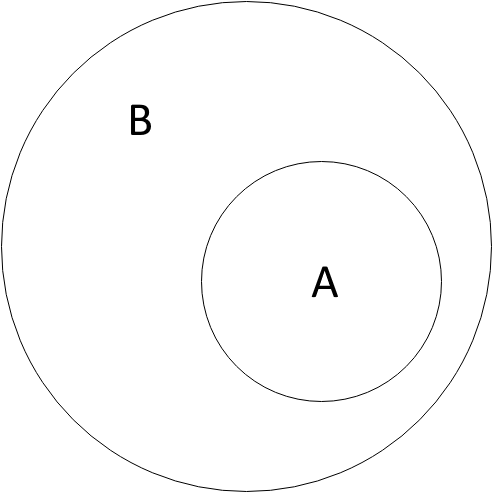
\includegraphics[width=\textwidth]{EulerCircles}
    \caption{Traditional Euler Circles}
  \end{minipage}
\end{figure}

Whilst according the Erickson the coincident are more commonly thought of, for diagrammatic purposes the traditional way will be discussed as it is clearer. As table 1.1 shows, when representing the individual moods Euler circles can be very intuitive.

%Cirles are 8.5cm I think
\begin{table}[h!]
  \centering
  \begin{tabular}{  c  c  c  c }
    A & I & E & O\\
    \begin{minipage}{.22\textwidth}
      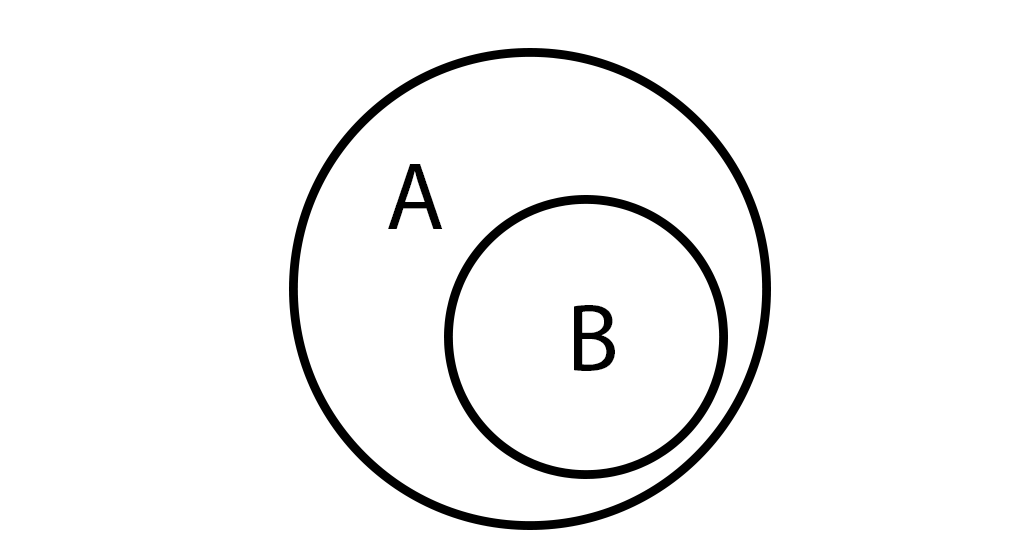
\includegraphics[width=\linewidth]{AEuler}
    \end{minipage}
    &
    \begin{minipage}{.22\textwidth}
      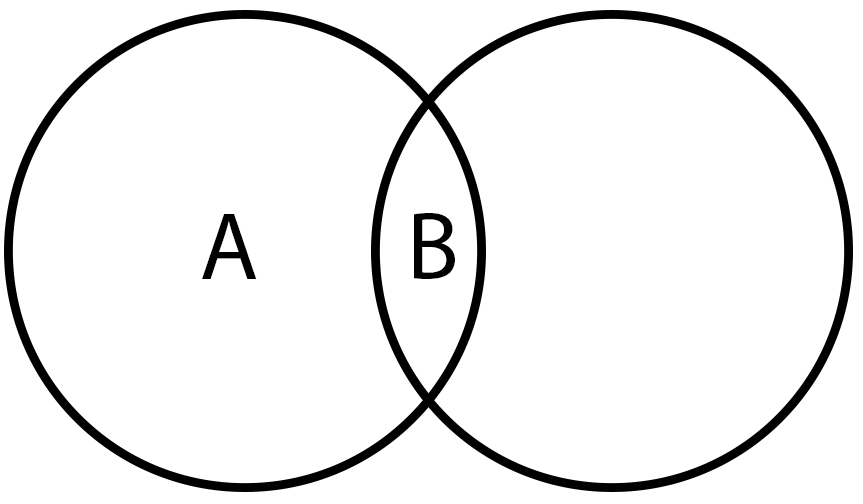
\includegraphics[width=\linewidth]{IEuler}
    \end{minipage}
    & 
    \begin{minipage}{.22\textwidth}
      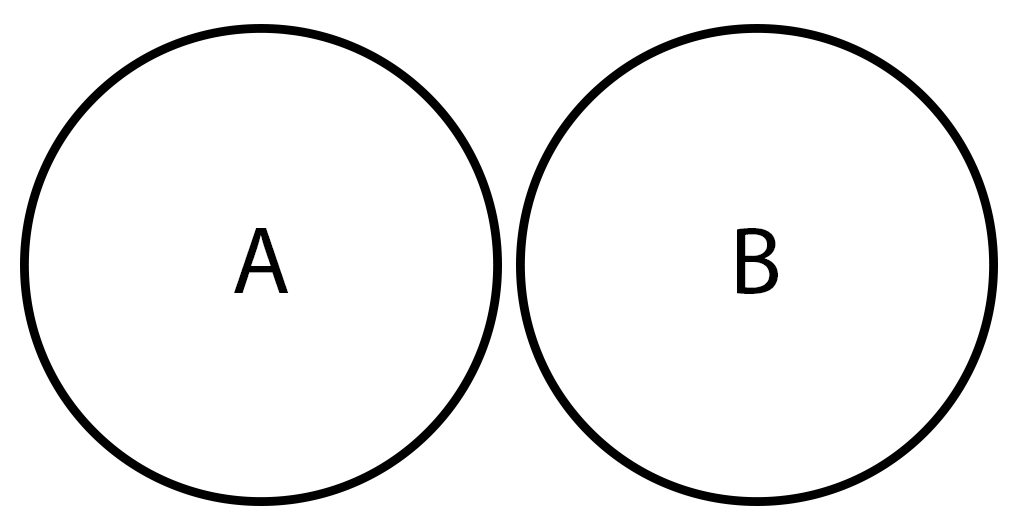
\includegraphics[width=\linewidth]{EEuler}
    \end{minipage}
    &
    \begin{minipage}{.22\textwidth}
      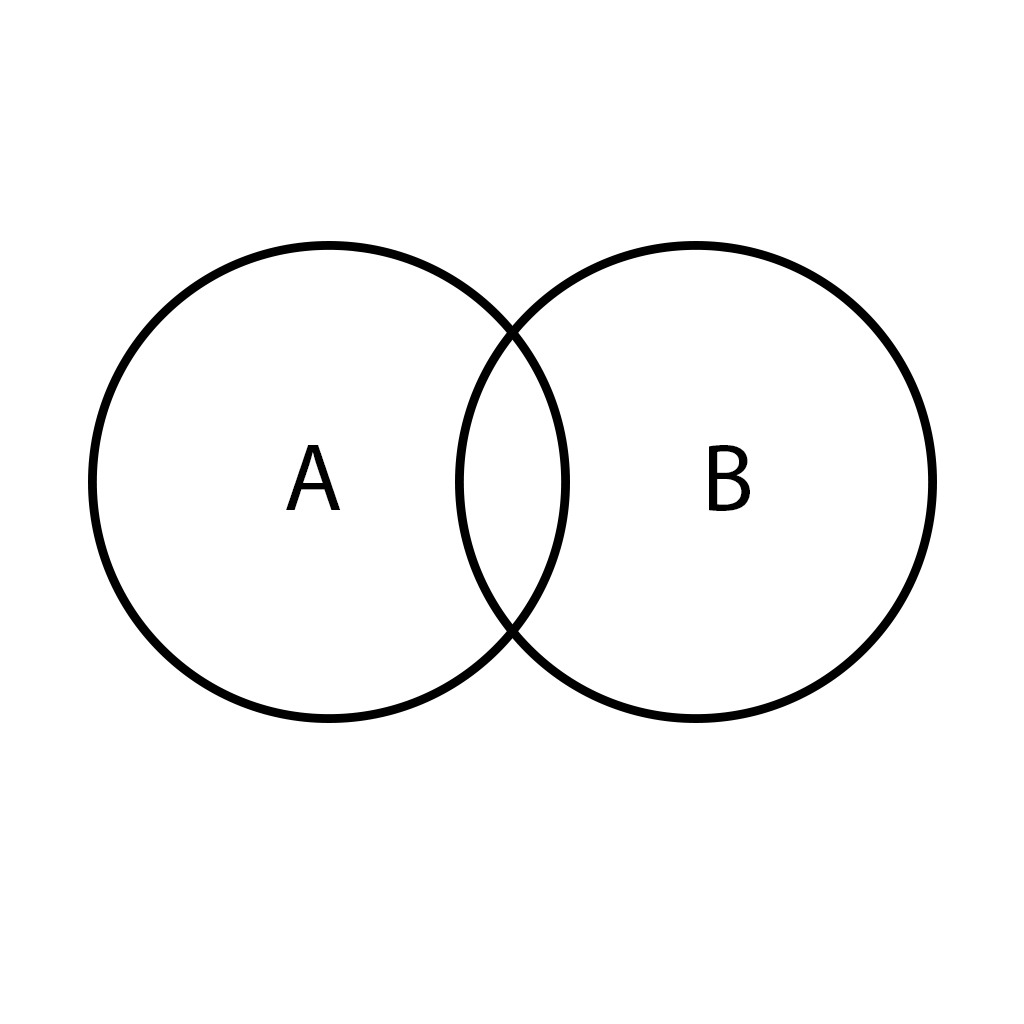
\includegraphics[width=\textwidth]{OEuler}
    \end{minipage}
    \\
  \end{tabular}
  \caption{Premises represented by Euler Circles}\label{tbl:eulerPremises}
\end{table}

\pagebreak
\noindent Euler circles also nicely represent simpler syllogisms are Table 1.2 shows.

\begin{table}[htb]
  \centering
  \begin{tabular}{ c  c  c }
    All Men Are Mortal & All Greeks Are Men & All Greeks Are Mortal\\
    \begin{minipage}{.29\textwidth}
      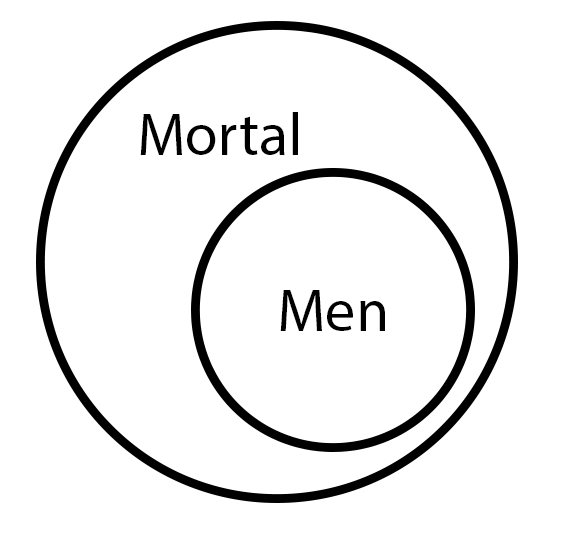
\includegraphics[scale=0.25]{EulerAllMenAreMortal}
    \end{minipage}
    &
    \begin{minipage}{.29\textwidth}
      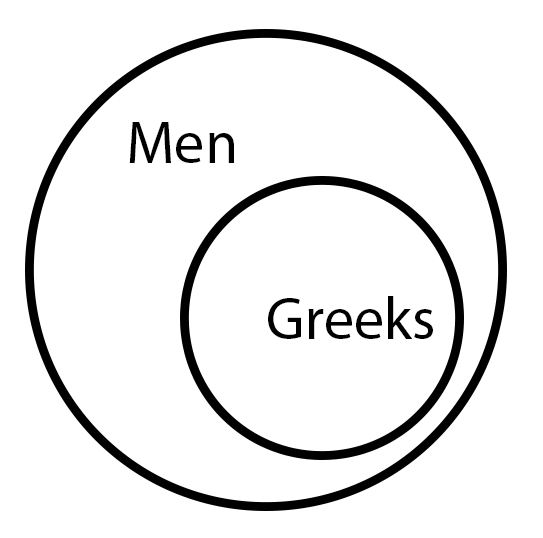
\includegraphics[scale=0.25]{EulerAllGreeksAreMen}
    \end{minipage}
    & 
    \begin{minipage}{.29\textwidth}
      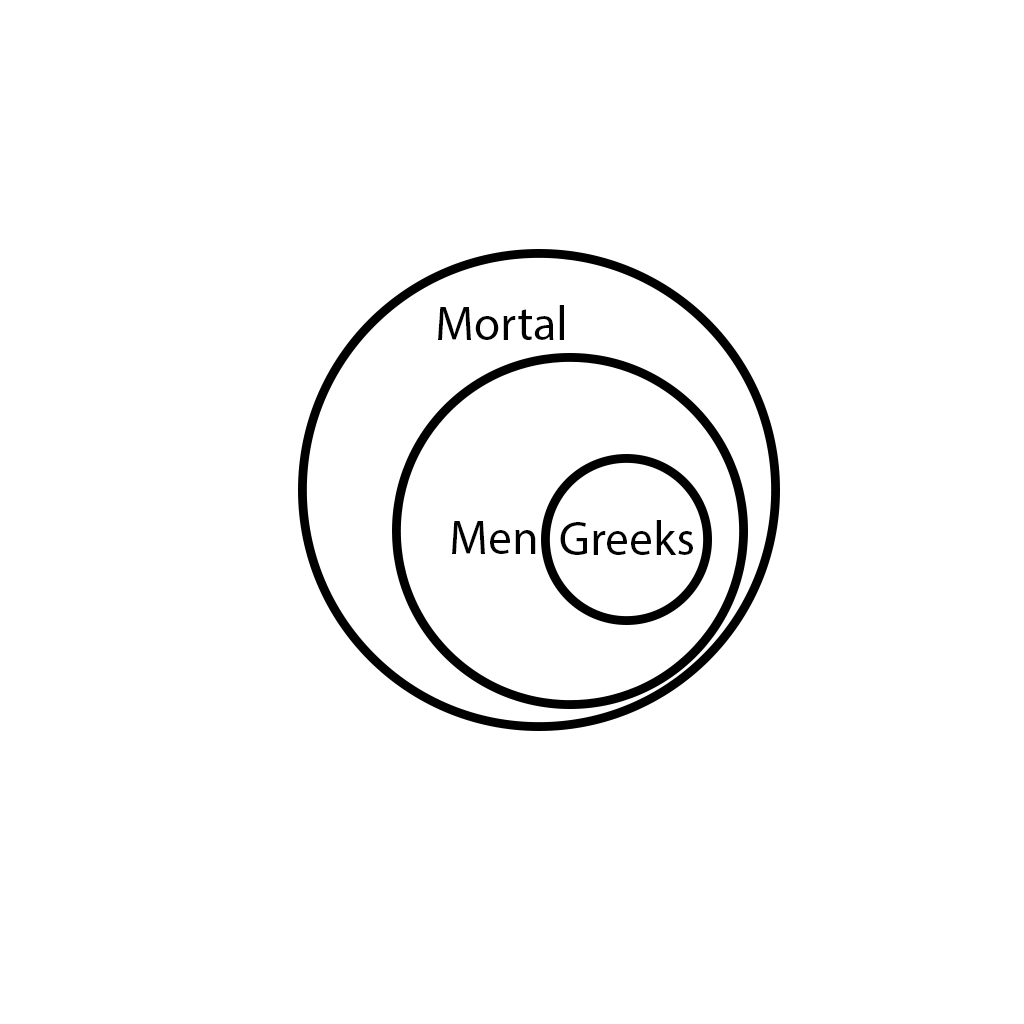
\includegraphics[scale=0.25]{EulerAllGreeksAreMortal}
    \end{minipage}
    \\
  \end{tabular}
  \caption{Premises represented by Euler Circles}\label{tbl:eulerPremises}
\end{table}
\FloatBarrier
However, the problem with this representation arises when more complex syllogisms are constructed. When there are multiple ways to represent the conclusion the resulst is needing more than one diagram to depict the possibilites. All of a sudden the intuitive benefits are quickly outweighed by the complexity.

\subsection{Venn Diagrams}
%Think about Plurative syllogisms for possible extensions
Venn diagrams are the most commonly used diagrammatic representation of syllogigms. A huge advantage of them is that most people have been taught them at a young age and are very familiar with them.

\begin{table}[h!]
  \centering
  \begin{tabular}{  c  c  c  c }
    A & I & E & O\\
    \begin{minipage}{.22\textwidth}
      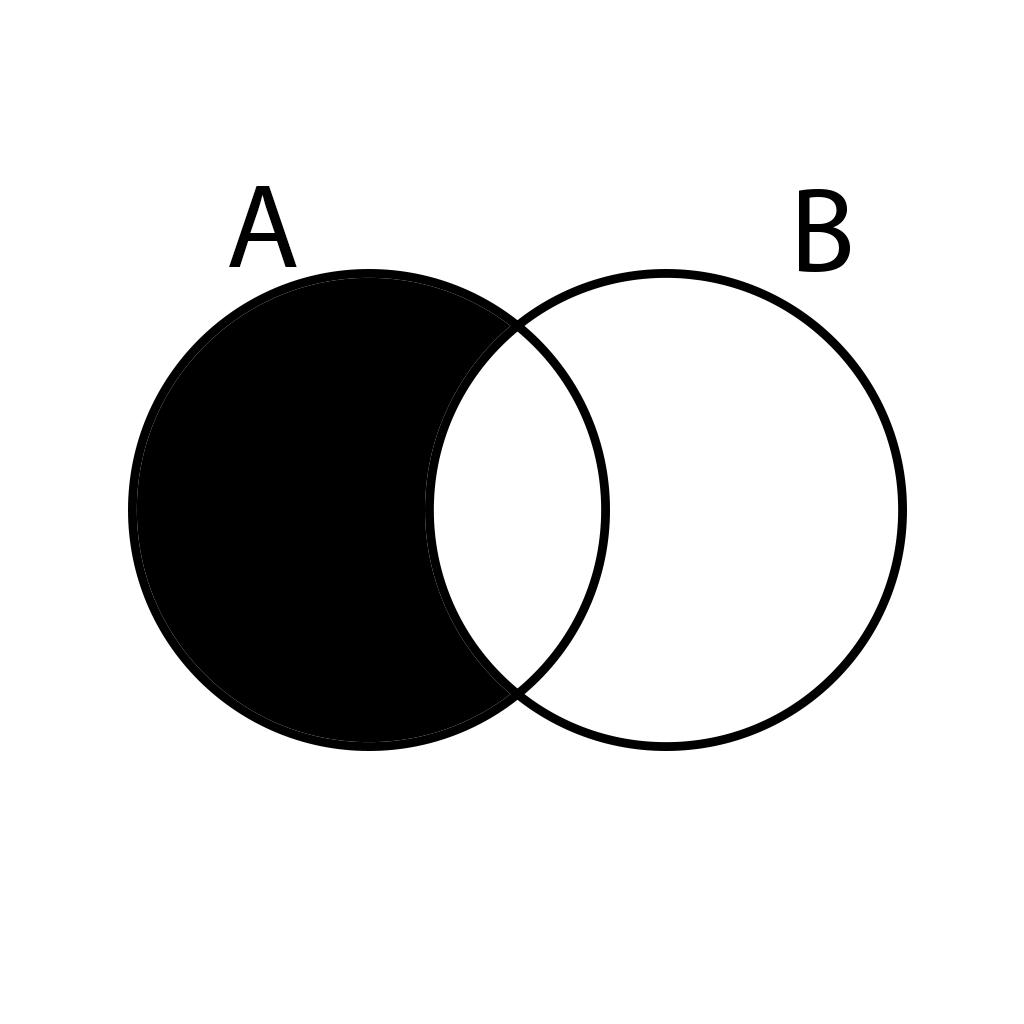
\includegraphics[width=\linewidth]{AVenn}
    \end{minipage}
    &
    \begin{minipage}{.22\textwidth}
      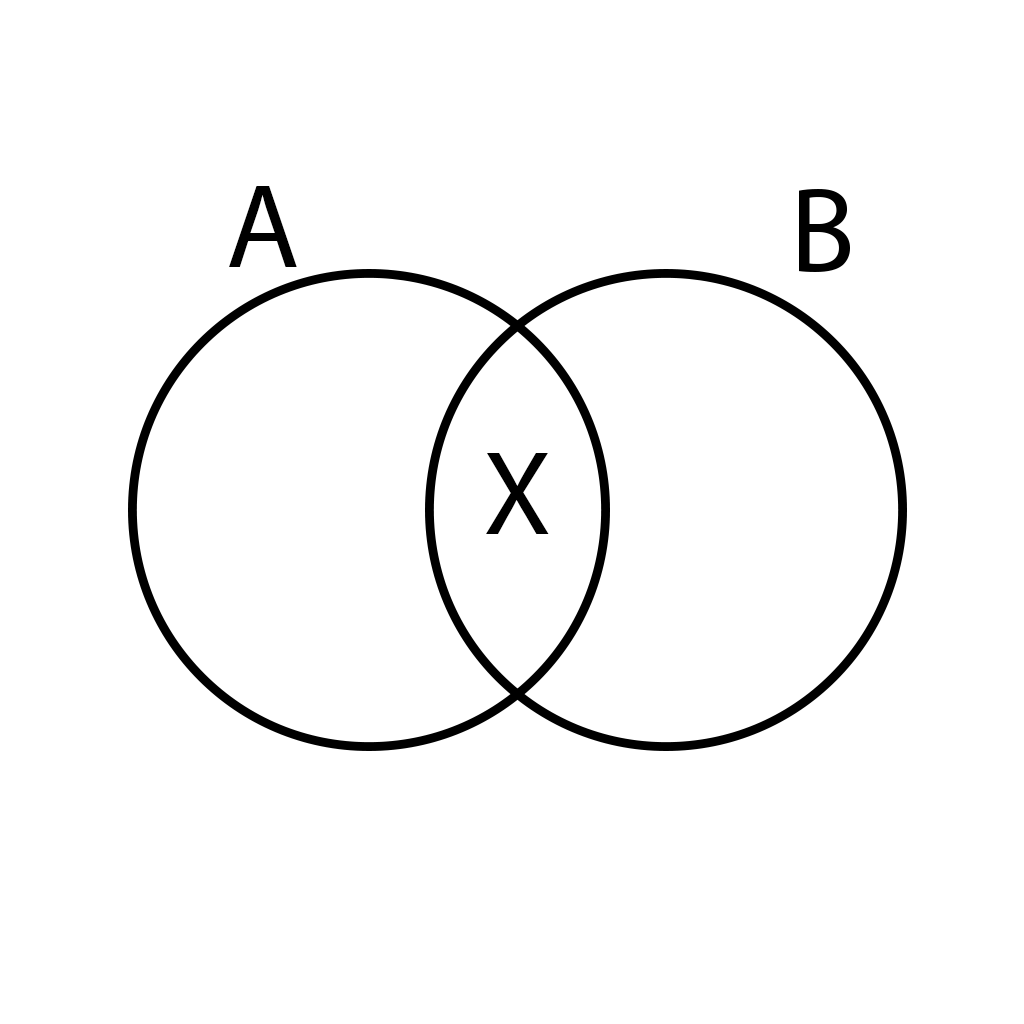
\includegraphics[width=\linewidth]{IVenn}
    \end{minipage}
    & 
    \begin{minipage}{.22\textwidth}
      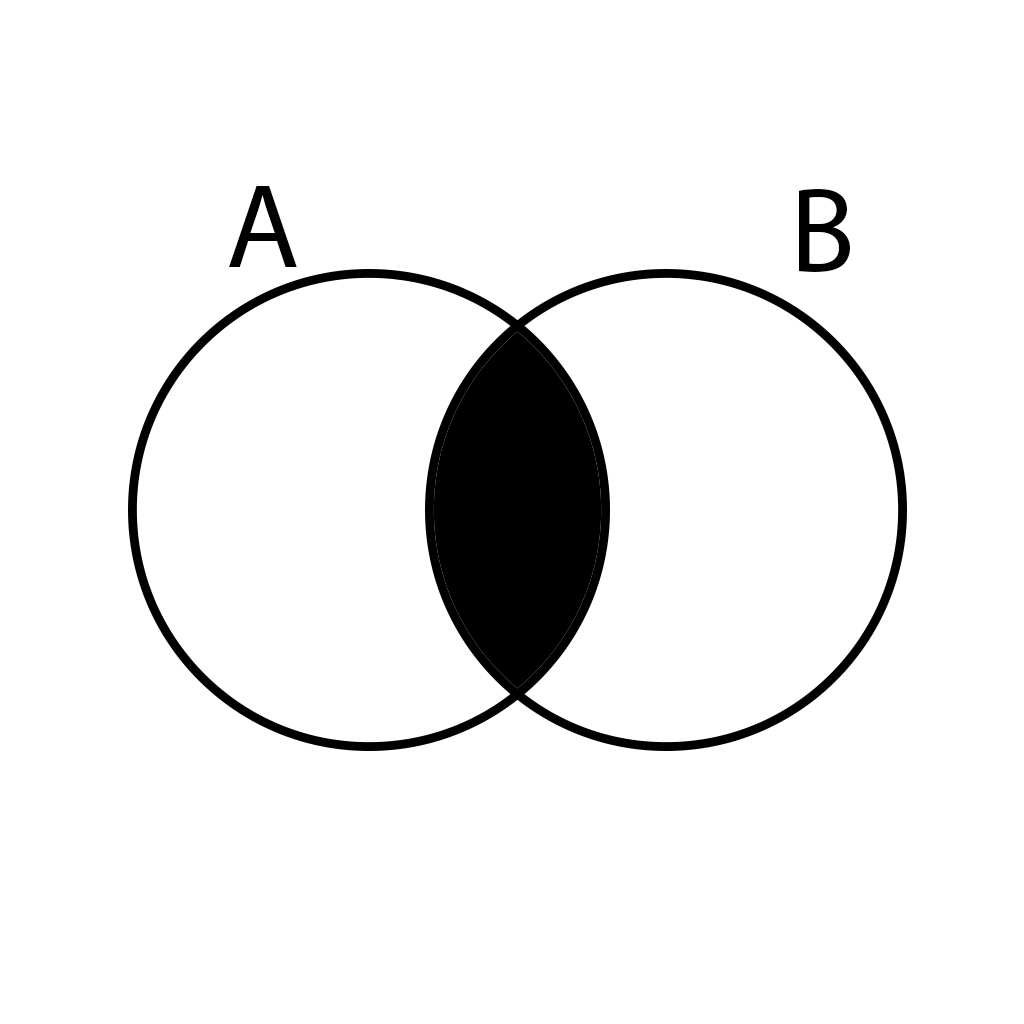
\includegraphics[width=\linewidth]{EVenn}
    \end{minipage}
    &
    \begin{minipage}{.22\textwidth}
      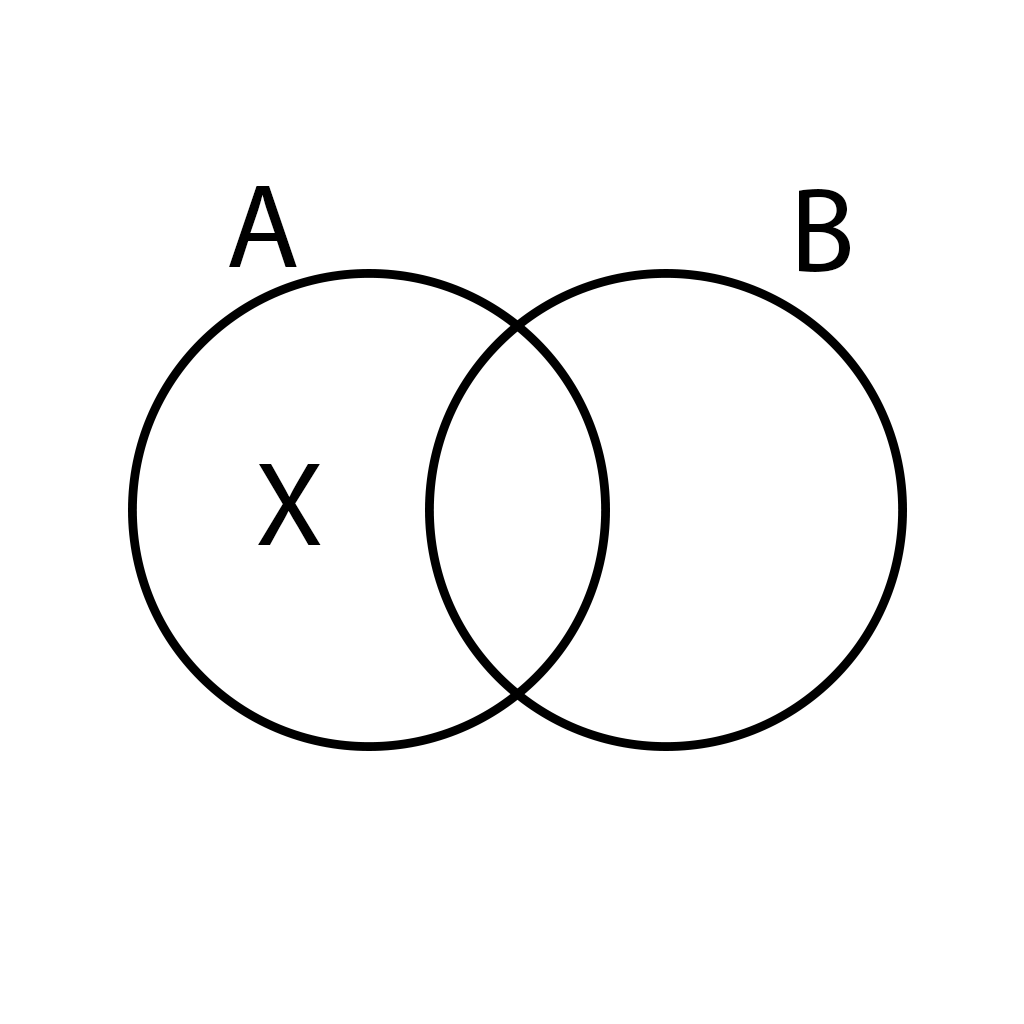
\includegraphics[width=\textwidth]{OVenn}
    \end{minipage}
    \\
  \end{tabular}
  \caption{Premises represented by Venn Diagrams}\label{tbl:eulerPremises}
\end{table}


\subsection{Linear Diagrams}
Linear diagrams are an alternative system that was devised by \cite{englebretsen1991}. Instead of being planar like Venn and Euler diagrams are linear. The reasoning behind this was that Englebretsen said it allowed linear diagrams to represent 4 terms, unlike their planar counterparts. Elements are represented by points which are then connected by lines to show sets.

%Cirles are 8.5cm I think
\begin{table}[h!]
  \centering
  \begin{tabular}{  c  c  c  c }
    A & I & E & O\\
    \begin{minipage}{.22\textwidth}
      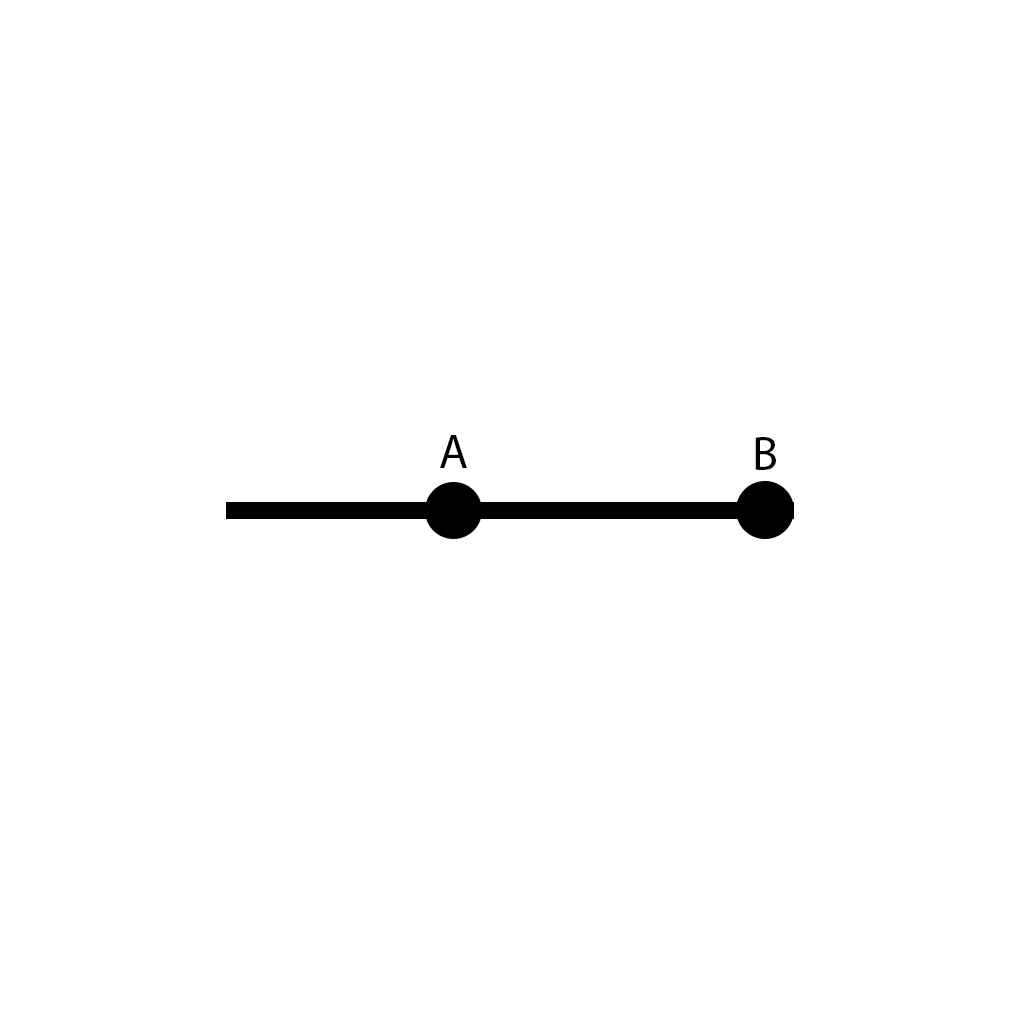
\includegraphics[width=\linewidth]{ALinear}
    \end{minipage}
    &
    \begin{minipage}{.22\textwidth}
      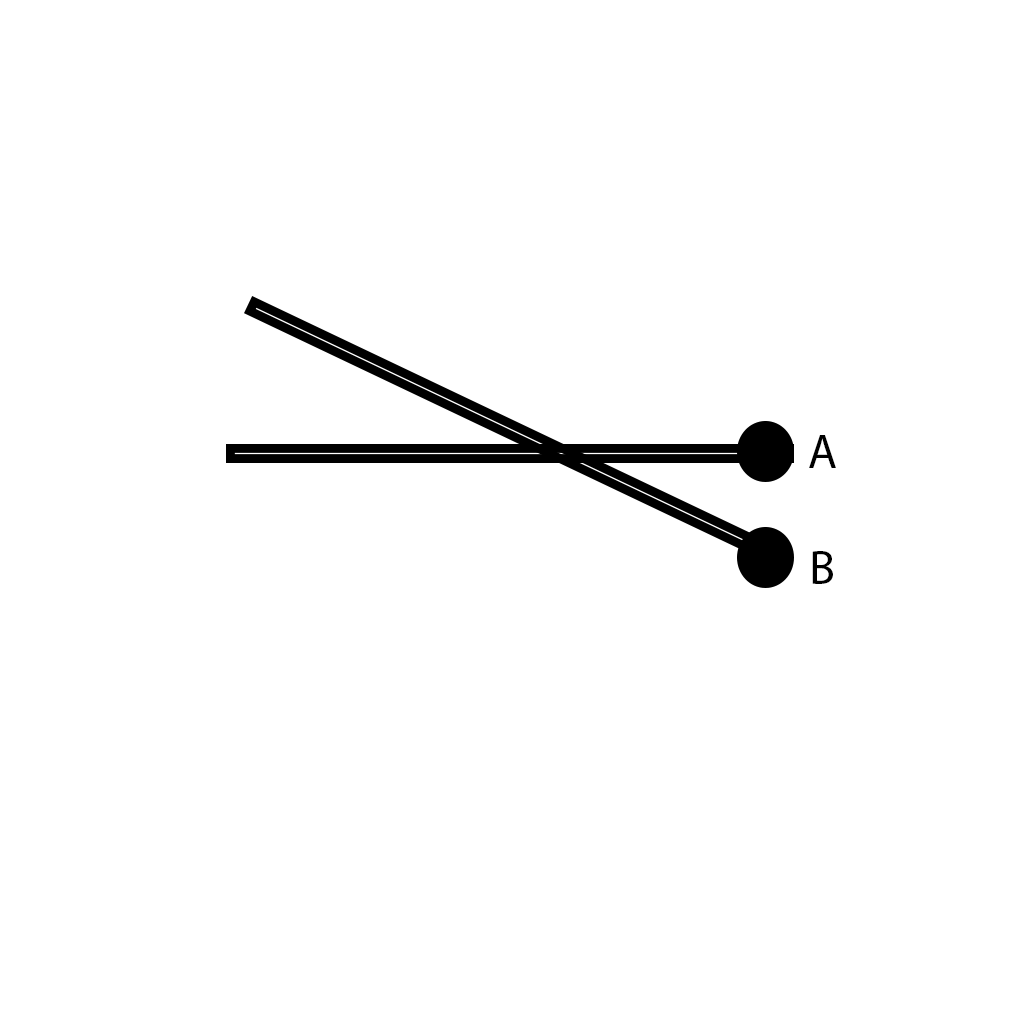
\includegraphics[width=\linewidth]{ILinear}
    \end{minipage}
    & 
    \begin{minipage}{.22\textwidth}
      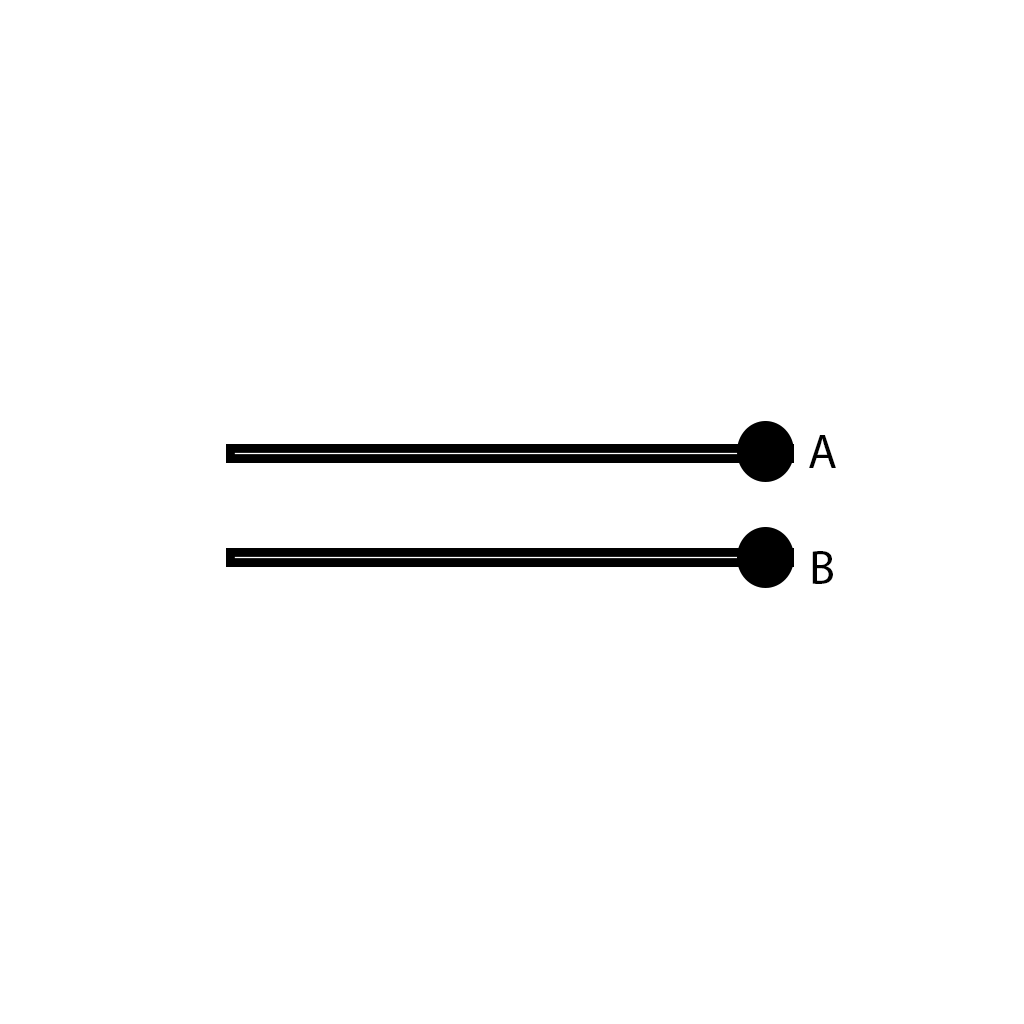
\includegraphics[width=\linewidth]{ELinear}
    \end{minipage}
    &
    \begin{minipage}{.22\textwidth}
      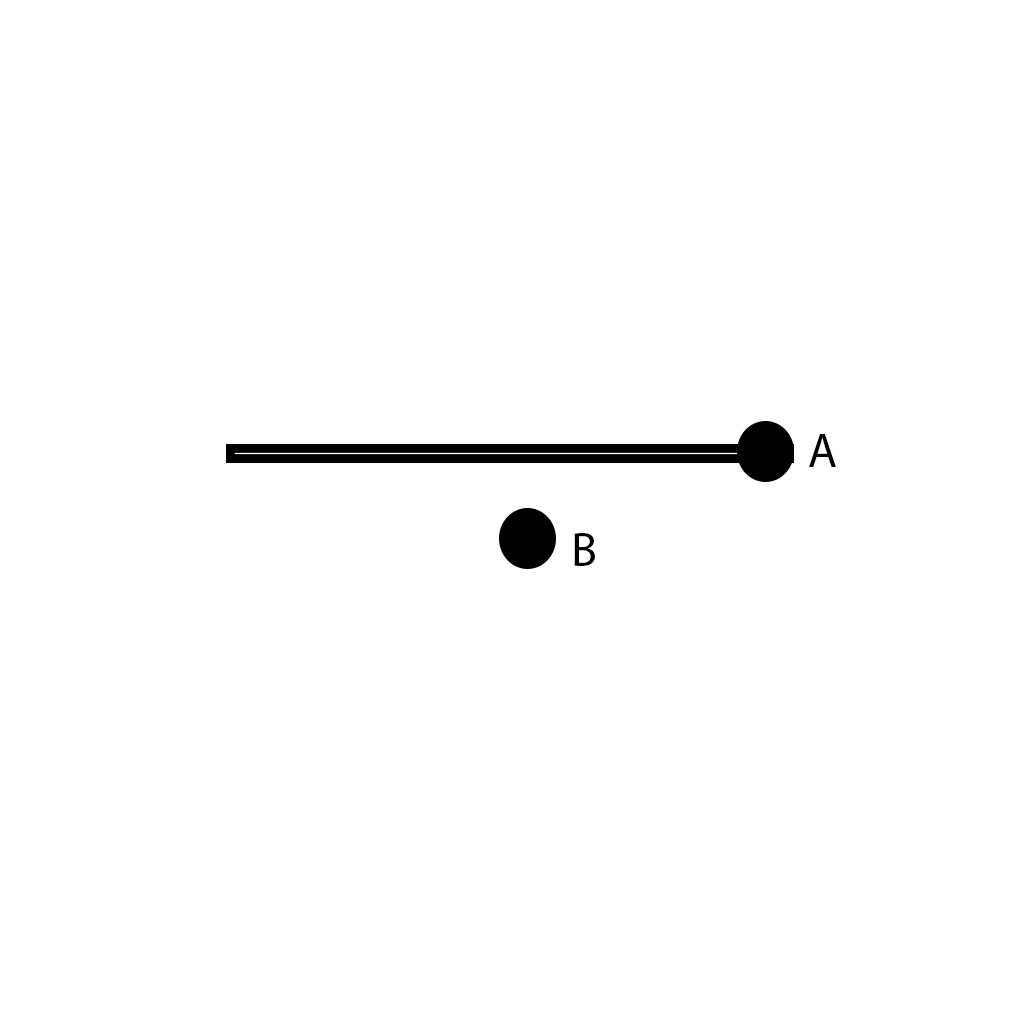
\includegraphics[width=\textwidth]{O1Linear}
    \end{minipage}
    \\
    &
     &
     &
    \begin{minipage}{.22\textwidth}
      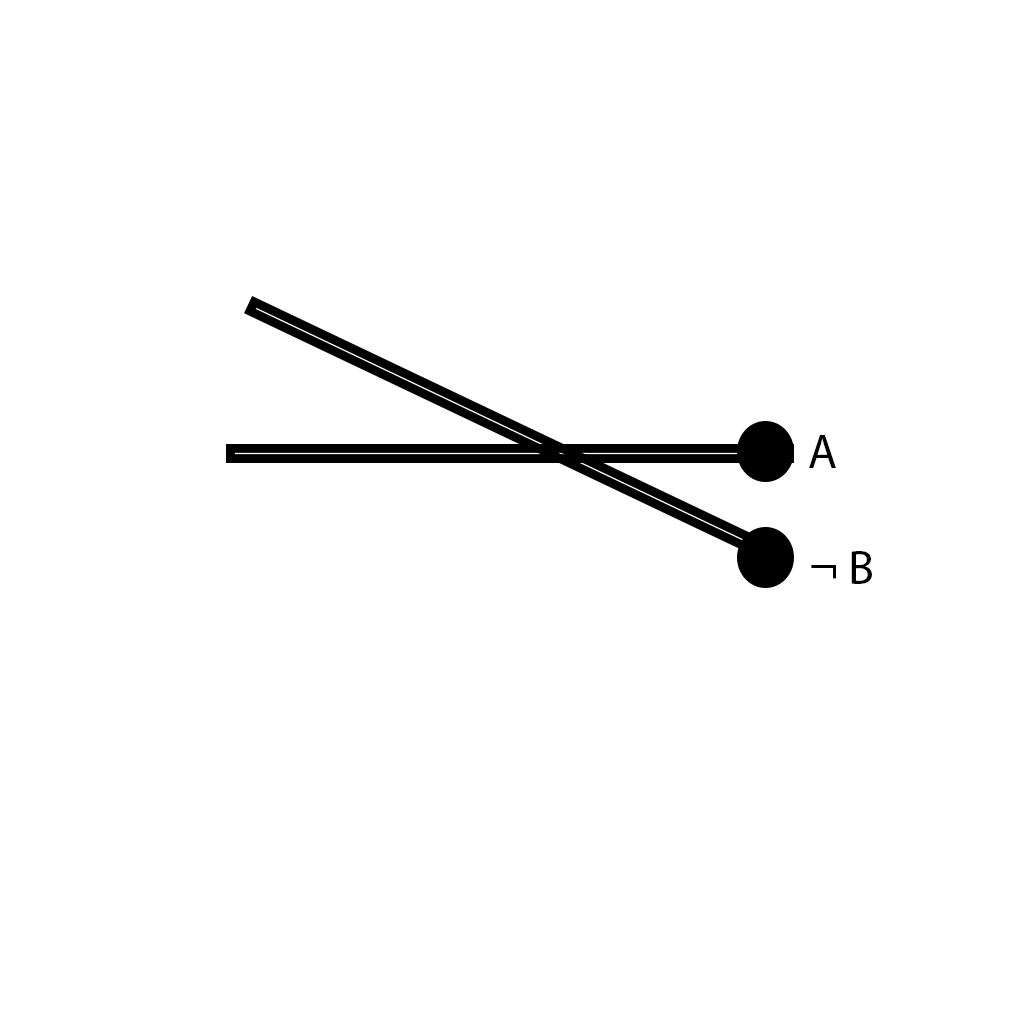
\includegraphics[width=\textwidth]{O2Linear}
    \end{minipage}
    \\
  \end{tabular}
  \caption{Premises represented by Linear Diagrams}\label{tbl:linearPremises}
\end{table}
\FloatBarrier

However, as shown by \cite{lemon1998insufficiency}, linear diagrams do not successfully manage to circumvent the same limitations that planar figures are susceptible to. 

\subsection{Categorical Pattern Diagrams}
As introduced by \cite{cheng2012visualizing}, Categorical Pattern Diagrams offer a relatively new approach with regards to representing syllogisms. The aim behind them is to simplify the process of checking validity, better represent syllogisms with more than 2 premises and generally make the diagrams easier to infer from.

The issue with this form of representation is the notation used is not intuitive. Categorical Pattern Diagrams require the person to learn a whole new notation before they can begin to reason about the syllogism that it is representing.

\chapter{Serious Games}
\section{Introduction}
Serious Games are a movement within the game industry comprised of software developers and researchers who are using games to educate. Whilst there is some debate around what exactly construes a serious game, \cite{michael2005serious} define one as any game where entertainment is not the primary purpose, but where instead the focus is on education. They aim to tackle a growing problem in education whereby educational techniques have not adapted to the needs of the current generation. As \citep{Lim} discusses, learning in the classroom has been driven by the national curriculum, with a massive focus on standard and grades. This goes against the belief that to engage students the focus should in fact be on creating a learning environment that encourages this.  In contrast with previous generations, the younger generation of today have grown up in a world consumed in technology. \cite{oblinger2005educating} described them as the \textit{Net Generation}, the generation who always need to be connected, require immediate feedback and crave social interaction. The research of \cite{prensky2001games} explains how this vast amount of technology now experienced in everyday life has led to these newer generations having their minds rewired. These cognitive changes have caused a different set of educational preferences when compared to previous generations, with teaching methods not evolving in order to take this into account.

\section{Why They Are Good For Education}
One of the benefits of using games to teach is their accessibility. In the United Kingdom  access to the internet has doubled over the past 10 years, with 82\% of adults now using the internet on a daily basis \citep{onssurvey}. With such a high number of people using the internet it allows games hosted on the web to be available to the masses. Games also appeal to a wide audience by crossing demographic boundaries such as age, gender and educational status \citep{griffiths2002educational}. 

\section{Existing Serious Games}
Serious Games can be split into two main categories, mini-games and complex games. Mini Games tends to be far shorter, often only taking less than an hour to complete, focussing on a very specific topic within a subject and browser based. Progression tends to be added through multiple levels, all with similar design but increasing the difficultly from previous levels. This is the far more common type of Serious Game as game development is extremely costly, and mini games allow implementation from as few as a single developer.

In contrast complex games can take potentially hundreds of hours to complete and cover a very broad topic. The game may contain multiple skills, paths to follow and complex goals. 

\section{Motivation}
As discussed by \cite{malone1981toward} games can also be intrinsically motivating, such that there are no external factors as to why a person is playing other than for their own enjoyment. This is in contrast to typical classroom learning that is usually more extrinsically motivated through grades, exam results and certificates. As  \citep{csikszentmihalyi1997talented} says, the number of students attending school would see a sharp drop if extrinsic rewards were removed. Of the two, intrinsic motivation is more resilient that extrinsic motivation. Learning that takes place as a result of intrinsic motivation if how higher quality of the knowledge is longer lasting \citep{kawachi2003initiating}. However, it is important to remember that not all games are by definition intrinsically motivating, but need to be structured correctly to achieve this. Malone included challenge, fantasy and curiosity as the three cornerstones of intrinsically motivating serious games.  In order to create a challenging game, it should include uncertain goals that are not too easy for the players to complete. Ensuring a game is challenging is so crucial as demonstrated by Malone through his work surveying children's opinion on 25 different computer games. The results conclusively showed that the most popular games all shared one thing in common; they all contained a defined goal.  Similarly in a study carried out by \citep{abuhamdeh2012importance} on chess players, it was found that the more challenging the game the greater the player's enjoyment. A fantasy environment in a game is said to "evoke mental images of phyical or social situations not actually present". Malone divides these fantasies into intrinsic and extrinsic, with intrinsic being more interesting and instructional resulting in a  greater cognitive effect on learning. \citep{lepper1988motivational} explains how if learning takes place away from the functionality of the knowledge then this decontextulisation results in the learner becoming demotivated.  This can be tackled by teaching topics by using real world examples demonstrating how the concepts are applied.  However, as this is not always feasible, Lepper proposed inserting the content of the topic into a fantasy context. Curiosity was the final and like challenge, is stimulated from an optimal level of complexity. Also similarly like fantasy, curiosity is  broken down into two categories; sensory and cognitive.  Sensory curiosity, as the name suggests, uses lights, sounds and graphics to gain that attention of the participant. Cognitive curiosity is achieved by making the participant doubt their existing knowledge, as people desire to have "good form" in their cognitive structure.   By using this taxonomy when developing a serious game, it is clear that this could be used to engage people who otherwise might not have been interested in learning. 

\section{Feedback}
Feedback is a crucial part of the education process and significantly influences the effectiveness of learning. Feedback in this context relates to information provided by a source, be it a teacher etc, regarding a person's understanding of a concept that be used to aid improvement.
As stated by \cite{hattie2007power}, "feedback is
one of the most powerful influences on learning and achievement".

One of the main advantages of using games for education is the speed at which feedback can be delivered to the learner. This is especially important to the \textit{Net Generation} who require this immediate feedback. For example, in the scenario of a teacher marking essays, it can be months between when the work was completed and when the feedback was received. The term \textit{Fast feedback} was coined by \cite{lumsden1988characteristics} which demonstrated how this timely feedback removed any uncertainty about progress and allowed any corrective action to be taken during the learning process.

The act of delivering feedback during the lenaring process is known as formative assessments, with summative assessments usually being carried out at the end. As explained by \cite{irons2007enhancing}, formative assessments can be hugely beneficial as they enhance the learning process by creating a positive environment which in turns results in greater motivation for learning. 

Serious Games lend themselves extremely well to delivering formative feedback to players through in-game features such as progress bars, score count and countdown timers. Feedback can also be provided to the player as they make mistakes allowing the player to engage with the game and keep on track to completing their goals. This can also help the player from becoming frustrated and not able to progress past a certain point.

\bibliographystyle{plainnat}
\bibliography{bibliography} 

\end{document}
